
%% Brewer_Sun.tex

\documentclass[journal]{IEEEtran}
%
% If IEEEtran.cls has not been installed into the LaTeX system files,
% manually specify the path to it like:
% \documentclass[journal]{../sty/IEEEtran}





% *** CITATION PACKAGES ***
%
\usepackage{cite}
% cite.sty was written by Donald Arseneau
% V1.6 and later of IEEEtran pre-defines the format of the cite.sty package
% \cite{} output to follow that of the IEEE. Loading the cite package will
% result in citation numbers being automatically sorted and properly
% "compressed/ranged". e.g., [1], [9], [2], [7], [5], [6] without using
% cite.sty will become [1], [2], [5]--[7], [9] using cite.sty. cite.sty's
% \cite will automatically add leading space, if needed. Use cite.sty's
% noadjust option (cite.sty V3.8 and later) if you want to turn this off
% such as if a citation ever needs to be enclosed in parenthesis.
% cite.sty is already installed on most LaTeX systems. Be sure and use
% version 5.0 (2009-03-20) and later if using hyperref.sty.
% The latest version can be obtained at:
% http://www.ctan.org/pkg/cite
% The documentation is contained in the cite.sty file itself.



\usepackage{array,tabularx}


% *** GRAPHICS RELATED PACKAGES ***
%
\ifCLASSINFOpdf
  \usepackage{graphicx}
  % declare the path(s) where your graphic files are
  \graphicspath{ {Images/} }
  \usepackage[justification=centering]{caption}
  % and their extensions so you won't have to specify these with
  % every instance of \includegraphics
  % \DeclareGraphicsExtensions{.pdf,.jpeg,.png}
\else
  % or other class option (dvipsone, dvipdf, if not using dvips). graphicx
  % will default to the driver specified in the system graphics.cfg if no
  % driver is specified.
  % \usepackage[dvips]{graphicx}
  % declare the path(s) where your graphic files are
  % \graphicspath{{../eps/}}
  % and their extensions so you won't have to specify these with
  % every instance of \includegraphics
  % \DeclareGraphicsExtensions{.eps}
\fi






% *** MATH PACKAGES ***
%
\usepackage{amsmath,float}



% IEEEtran contains the IEEEeqnarray family of commands that can be used to
% generate multiline equations as well as matrices, tables, etc., of high
% quality.






% correct bad hyphenation here
\hyphenation{op-tical net-works semi-conduc-tor}


\begin{document}
%
% paper title
% Titles are generally capitalized except for words such as a, an, and, as,
% at, but, by, for, in, nor, of, on, or, the, to and up, which are usually
% not capitalized unless they are the first or last word of the title.
% Linebreaks \\ can be used within to get better formatting as desired.
% Do not put math or special symbols in the title.
\title{\LaTeX Generation from Printed Equations}
%
%
% author names and IEEE memberships
% note positions of commas and nonbreaking spaces ( ~ ) LaTeX will not break
% a structure at a ~ so this keeps an author's name from being broken across
% two lines.
% use \thanks{} to gain access to the first footnote area
% a separate \thanks must be used for each paragraph as LaTeX2e's \thanks
% was not built to handle multiple paragraphs
%

\author{Jim~Brewer, James~Sun
        \\
        Department of Electrical Engineering\\
        Stanford University\\
        Stanford CA, 94305\\
        Email: \{jebrewer, jsun2015\}@stanford.edu}


% make the title area
\maketitle

% As a general rule, do not put math, special symbols or citations
% in the abstract or keywords.
\begin{abstract}
This article describes a system that takes a photograph of a printed equation and produce a \LaTeX code representation. The process uses adaptive thresholding with mean filtering, morphological edge smoothing, and the Hough transform for image binarization and skew correction. The project uses Hu invariant moments and circular topology to match characters against a database of characters. The algorithm then assembles the appropriate LaTeX code from the detected characters. This system is able to detect 93.6\% of characters in “ideal” images and 86.2\% of characters in real-world photographs when combining two different skew methods (74\%-79\%).
\end{abstract}



\section{Introduction}
% The very first letter is a 2 line initial drop letter followed
% by the rest of the first word in caps.
% 
% form to use if the first word consists of a single letter:
% \IEEEPARstart{A}{demo} file is ....
% 
% form to use if you need the single drop letter followed by
% normal text (unknown if ever used by the IEEE):
% \IEEEPARstart{A}{}demo file is ....
% 
% Some journals put the first two words in caps:
% \IEEEPARstart{T}{his demo} file is ....
% 
% Here we have the typical use of a "T" for an initial drop letter
% and "HIS" in caps to complete the first word.
\LaTeX is a powerful typesetting system that is extremely useful for technical documents, particularly mathematical equations. However, once rendered, the output cannot be modified without access to the underlying code. Re-coding lengthy equations is time consuming and prone to errors. The ability to take a photograph of an existing equation printed in a textbook, homework assignment or technical article and to produce the editable \LaTeX code solves this problem. The challenges to accomplishing this involve cleanly converting the photograph to a binary image, correcting skew from the horizontal, correctly segmenting each individual character, matching the characters to a database of characters, and finally placing generating the correct \LaTeX representation of the equation.

\section{Related Work}
The advent of smartphones has prompted the rise of applications that automatically recognize and solve mathematical equations using a built in phone camera; one example is the popular PhotoMath application. However, less work has gone into translating equations into \LaTeX code.\\
The problem of character recognition has also seen numerous techniques that have had varying levels of success. Examples include the basic template matching algorithm using morphological operators or additional character properties\cite{Naqvi:article_typical}. Some have used morphological operators with only portions of the character to reduce the dataset and detect characters based on certain combinations of matched operators\cite{Pradhan:article_typical}. Others have used various region-based invariant moments such as the Hu, Zernike, and Krawtchouk moments\cite{Potocnik:article_typical} and circular topology of individual characters in an effort to have scale, translation, and rotation robustness \cite{Torres-Mendez:article_typical}. This project combines the use of the Hu moments with circular topology.

\section{Process Flow}
The following processing pipeline converts an image of an equation to \LaTeX code, see below. First, the image is captured; the target use-case does this through a smartphone camera, typically this was done with a smart-phone camera with the image then sent to laptop or desktop running MatLab to process the image and output the final code. Next, the image was is binarized with a white background and black characters. Then, any  skew to the image was detected and is corrected so the equation  in the image is horizontalwas oriented on the horizontal. Afterwards, Ssegmentation algorithms were then applied to find each individual contiguous character in the equation to then have an, extract a identifier feature vector, and extracted and run through a identify the character using nearest neighbor classifier to determine a character matchcation. Finally, the matched characters and their relative positions, from the segmentation algorithm, are used toan algorithm  assemble the final equation and output assembles the recognized characters into \LaTeX code. The current implementation of the process outputs the resultant code as a a .tex file that could be directly compiled or copied into an existing \LaTeX document.to be used as needed.
The following sections describe each part of the pipeline in more detail.

\subsection{Binarization}
The input RGB image is first converted into a binary image for processing. We found that treating scanned images differently from smartphone photographs gave the best results. In order to differentiate between the two image types, an image is first converted to grayscale. Then, we look at the proportion of pixels that are mid-gray, defined as having an 8-bit intensity value between 15 and 240, inclusive. If this proportion is less than 0.1, we classify the image as a scanned or screenshotted image; otherwise, we classify the image as a photograph. The following two sections describes the binarization method carried out for each class of image.
\subsubsection{Smartphone Photographs}
Photographs taken by a smartphone invariably contain uneven lighting and page imperfections. We perform adaptive thresholding with noise removal to compensate. First, the image is blurred with a Gaussian filter to smooth edges and remove high frequency noise, if the image is high-resolution. This pre-filtering is very beneficial for character recognition in high-resolution images but actually has a detrimental effect for low-resolution images due to the small number of pixels in the image. We empirically determined that an image with more than $2000\times1000$ pixels is well classified as high-resolution for use with a $10\times10$ Gaussian filter with standard deviation of $3$.

We use adaptive thresholding for the actual binarization in order to compensate for uneven lighting. The window size is set at $1/60^{\text{th}}$ of the smaller dimension of the image. This adaptive window size was chosen in order to adequately handle uneven lighting while still being small enough to preserve the integrity of most of the characters. To eliminate the overhead of performing Ostu’s method on each window, we leverage the fact that each image consists only of black text or white background. Thus, we use the $\text{window mean}-10$ as the threshold, with the offset of 10 to eliminate the effect of noise in the background. The window means are calculated quickly by convolving with an averaging filter; subtracting the offset from the output creates our thresholds matrix. Then, we take the difference of the image and the thresholds, allowing us to produce the binary image by thresholding this difference matrix with $0$.

After producing the binary image, we invert it so that the foreground is now the text and noise. We remove the noise in the background by performing an area opening operation. Afterwards, we perform a closing operation to close gaps in character edges. Finally, since the chosen window size may have created gaps in the middle of some characters with thick strokes, we perform small hole filling. Afterwards, we return the output image to the original polarity in order to obtain the final binarized output.

\subsubsection{Scanned and Screenshotted PDFs}
 Scanned and screenshotted PDFs should not need to have lighting correction performed. To prevent excessive runtime and unnecessary distortion, we perform Otsu’s method for these images.
 
 \subsection{Skew Correction}
 We then correct the binarized image for rotations. To compute the dominant orientation, we take the Hough transform. Luckily, most equations have multiple horizontal lines, such as fraction bars, equal signs, and negative signs, as seen below. This means that the dominant orientation is usually given by the correct, horizontal orientation. In order to guard against large magnitude peaks given by long diagonal lines such as the diagonal division bar in Figure \ref{fig:1}, we consider the top four magnitude Hough peaks and choose the mode of the orientations. 
 
 \begin{figure}[!t]
    \centering
    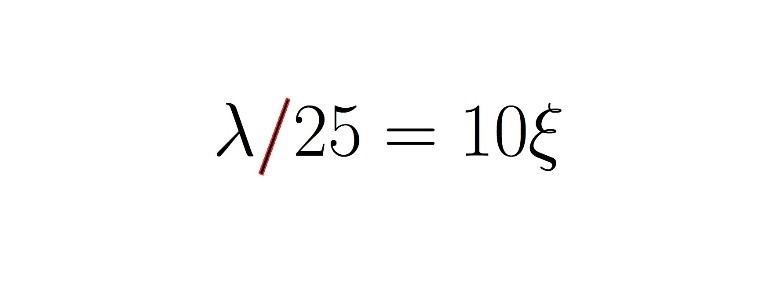
\includegraphics[width=\columnwidth]{fig1}
    \caption{Image with Problematic Non-Horizontal Line}
    \label{fig:1}
 \end{figure}
 
 Also, while the image in Figure \ref{fig:2} is rotated by a small positive angle, the orientation in Hough space is given as the angle between the normal and the horizontal axis, which is the complement of our desired angle. 
 
\begin{figure}[!t]
  \centering
  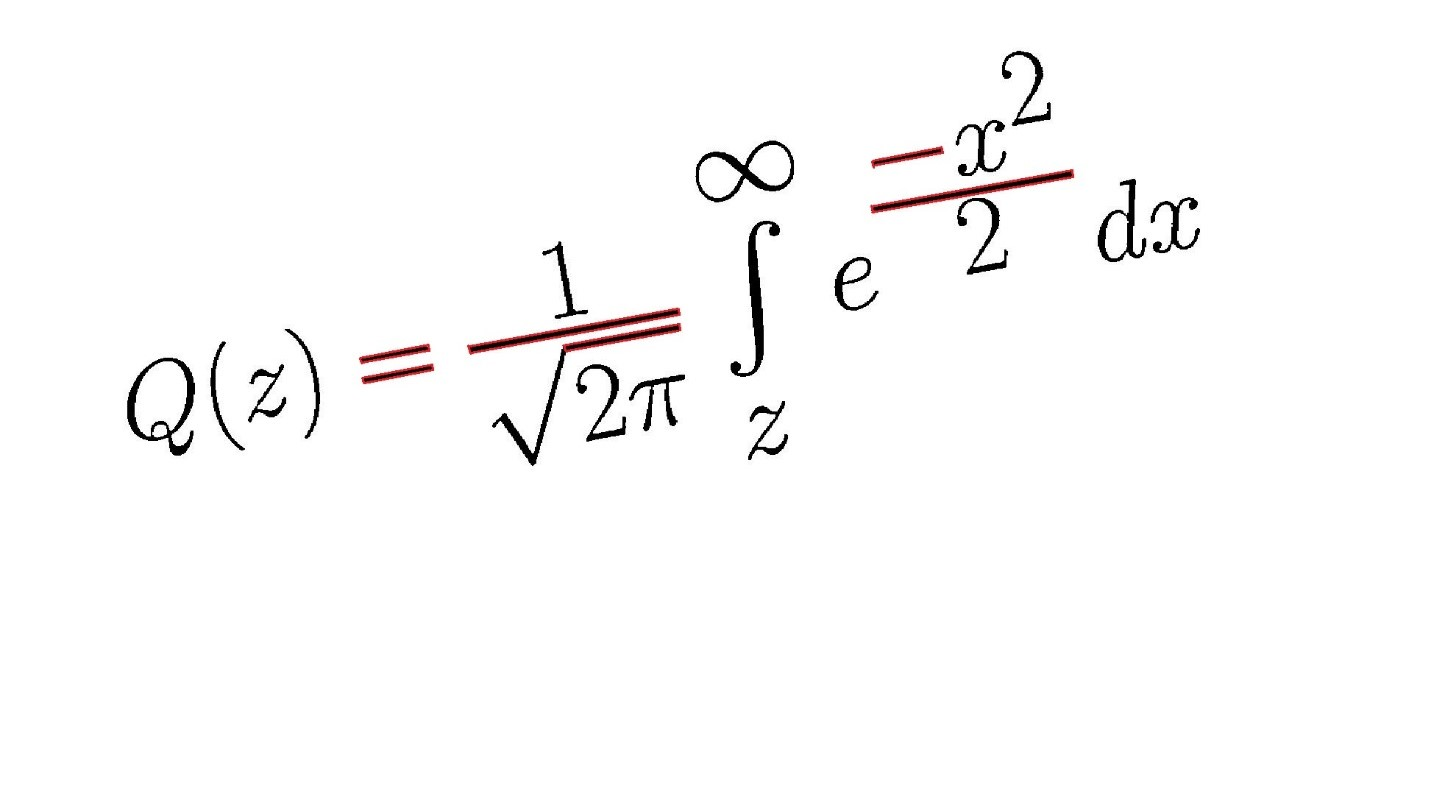
\includegraphics[width=\columnwidth]{fig2}
  \caption{Skewed Binarized Image}
  \label{fig:2}
\end{figure}
 
 For visualization, in Figure \ref{fig:3}, we want θ, but the Hough transform gives us ρ, but we correct for this easily by subtracting 90ᵒ. More importantly, after derotating the image, we perform edge softening if the detected rotation angle is significantly large. Significant rotations introduce quantization errors along straight lines, manifesting in jagged edges that are detrimental to character recognition. Currently, we soften the edges using an opening operation (we use opening because the image text is the background). The output of the Skew Correction algorithm is fed into the Segmentation algorithm of the Character Matching portion of the pipeline, described in the next section.
 
 
 
\begin{figure}[!t]
    \centering
    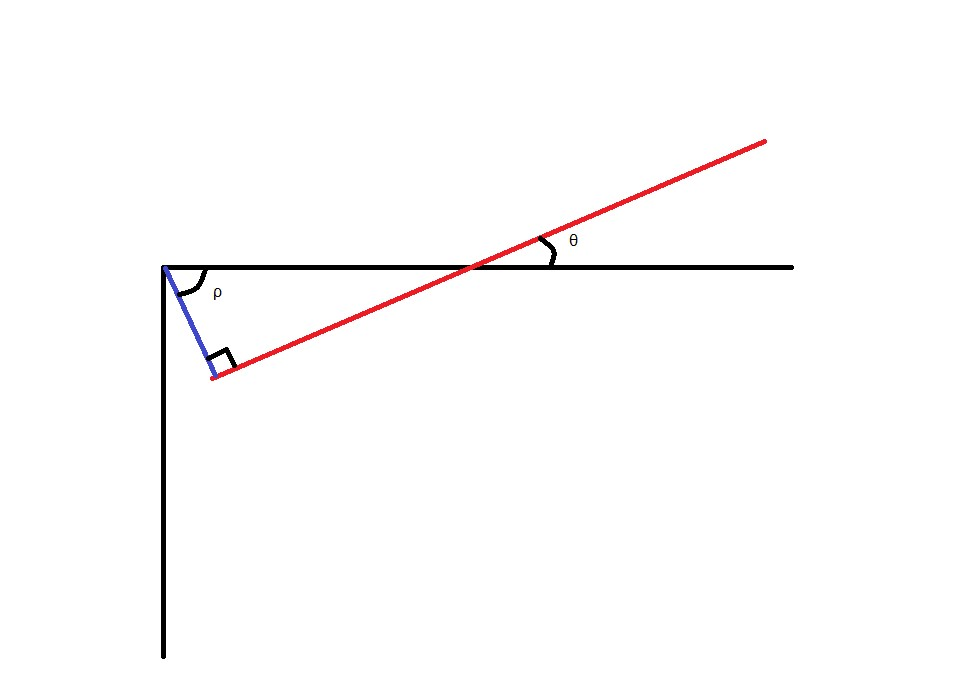
\includegraphics[width=\columnwidth]{fig3}
    \caption{Skew angles}
    \label{fig:3}
\end{figure}
 
\subsection{Segmentation}
Because characters are matched individually, the characters are first extracted from the derotation algorithm output. We considered several approaches, such as recursive segmentation\cite{Naqvi:article_typical}, but decided to use centroids and bounding boxes of edge maps for simplicity and for the ability to extract characters surrounded by others (such as a square root).
First, the edge map is obtained by eroding the inverted image and then XORing that with the original inverted image, resulting in a white edge map on a black background. Then, for each edge, we extract its centroid, bounding box and convex hull. This successfully extracts many characters, but we must still handle numerous edge cases. For example, this method can produce extraneous segmentations with characters such as $B$ that have inner contours, as shown in Figure \ref{fig:B}.

\begin{figure}[!t]
    \centering
    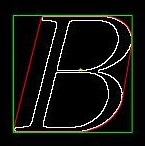
\includegraphics{B}
    \caption{Segmented $B$}
    \label{fig:B}
\end{figure}

Thus, if a character’s convex hull is fully contained within another convex hull, we examine the edges of to determine if the outer character fully surrounds the inner character. If so, we discard the inner segmentation. This additional edge check is necessary before discarding the inner segmentation for equations with a square root symbol, such as in Figure \ref{fig:seg_eq} where the characters underneath the square root are completely within its bounding box. 

\begin{figure}[!t]
    \centering
    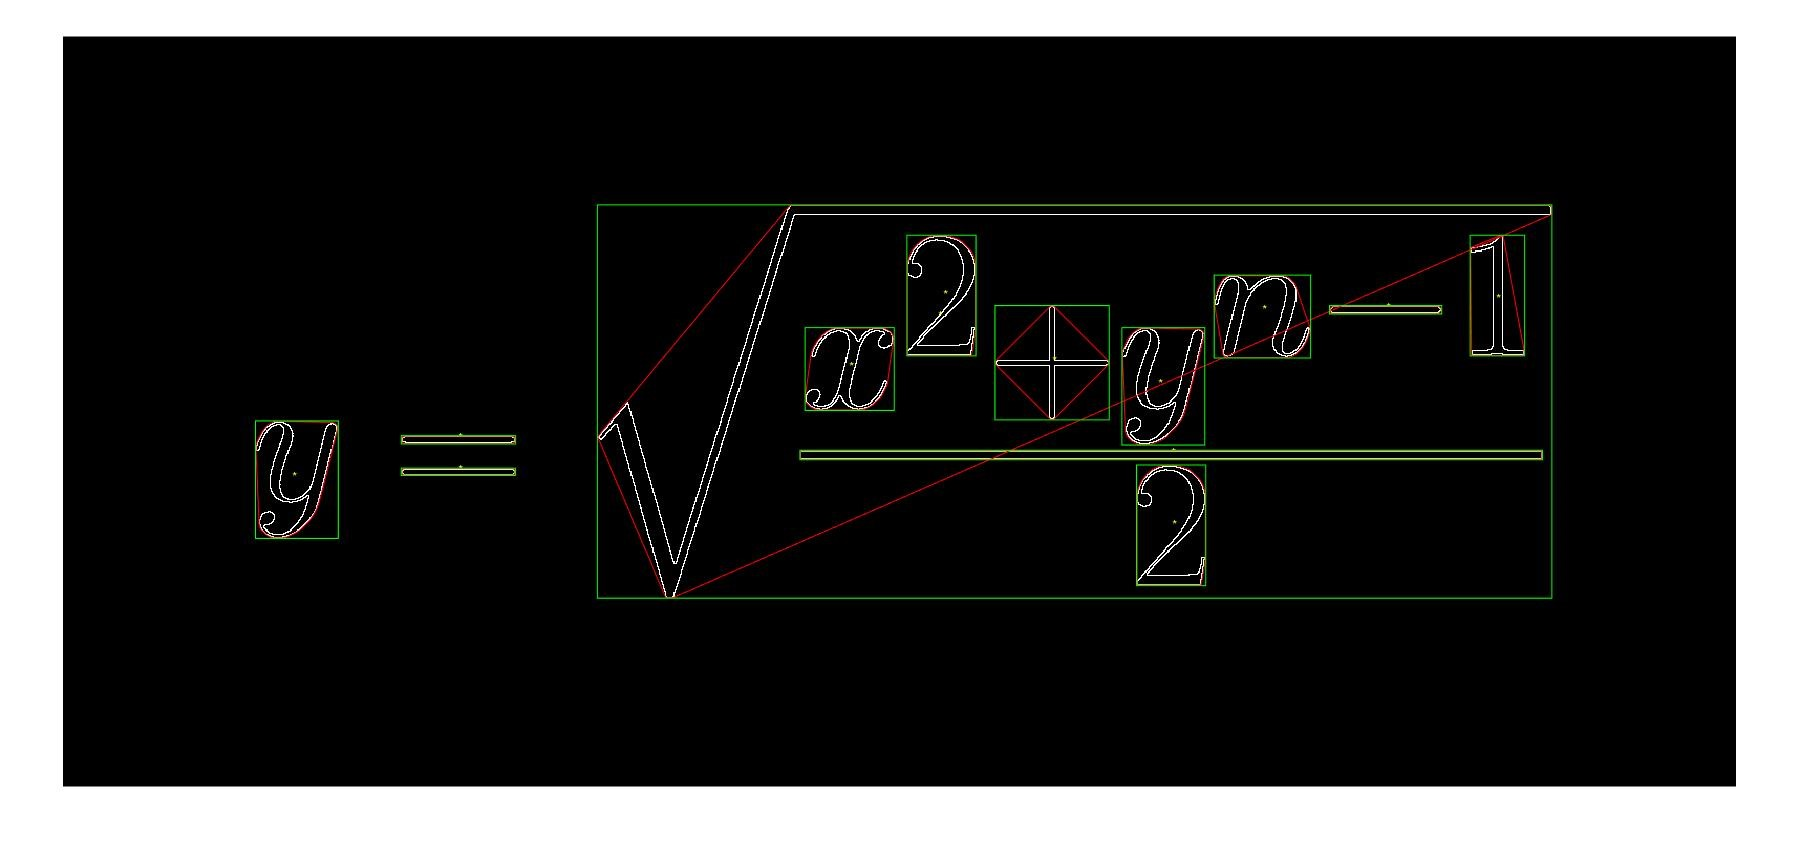
\includegraphics[width=\columnwidth]{seg_eq}
    \caption{Segmented Square Root}
    \label{fig:seg_eq}
\end{figure}
Finally, we extract each bounding box region and keep the largest single character within each one.

\subsection{Character Identifier}
Afterwards, we build an identification profile for each segmented character. The identification profile is a twenty-two element vector to be used to match the segmented character with a match in the template database.
We chose these characteristics to be invariant to translation, scaling, and rotation. Specifically, we integrated the usage of the following features that have been used in separately in literature:  the normalized central moment of inertia, circular topology\cite{Torres-Mendez:article_typical}, and Hu Invariant Moments\cite{Potocnik:article_typical}.
The first element in the vector is the normalized central moment of inertia\cite{Torres-Mendez:article_typical}. The central moment of inertia is translation- and rotation-invariant; normalization renders it scale-invariant. The following equation calculates this:
\begin{center}
    
\(
I_N = \frac{\sum\limits_{i=0}^N((x_i-c_x)^2 + (y_i - c_y)^2)}{N^2}
\)
\end{center}
where $N$ is the total number of character pixels in the image, and $c_x$ and $c_y$ are the coordinates of the character’s centroid.

The next fifteen elements are extracted from circular topology. Since the circle is geometrically rotationally invariant, the topology of the character along a circular path is likewise invariant. Eight circles centered at the character’s centroid but with varying radii are placed over the character. We determine the spacing of the circles by finding the maximum distance from the centroid to an edge of the character and then dividing by $k+1$ where $k$ is the number of circles. We used $k=8$ based on empirical results and previous literature. The first eight elements of these topology elements are the number of times each circle crosses the character.

Note that we used $k+1$ as the spacing but only considered the first $k$ circles. We found that having the outer circle on the edge of the character created topological aliasing errors due to imperfections on the character edges. Morphological opening operators were able to combat aliasing to some extent for other edge cases.

\begin{figure}[!t]
    \centering
    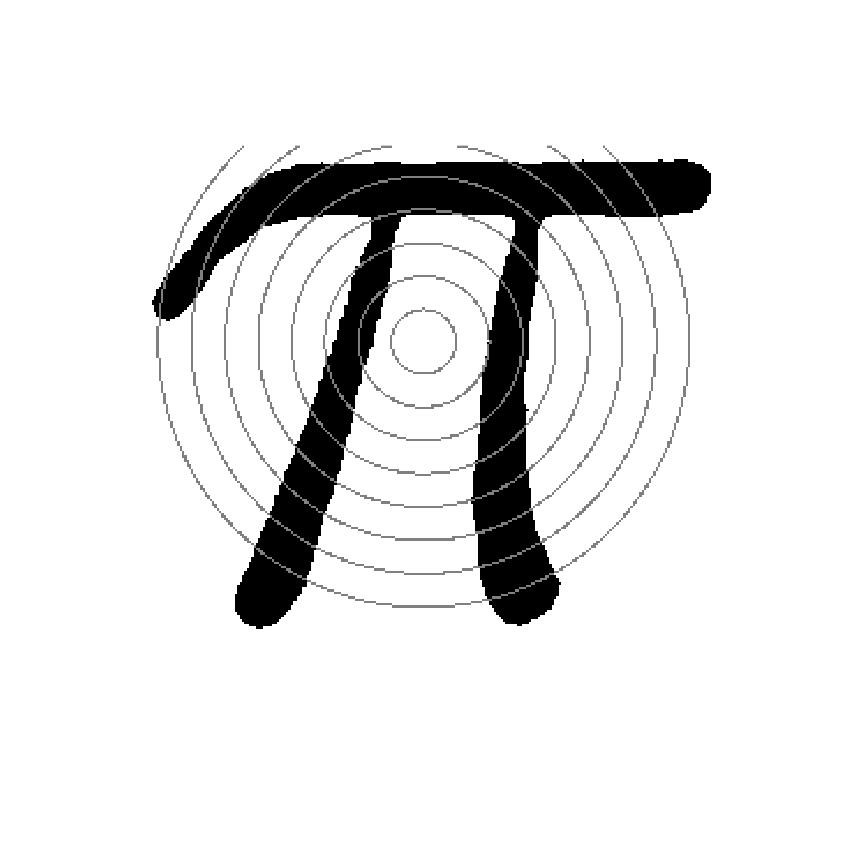
\includegraphics[width=\columnwidth]{pi_hu}
    \caption{Count: $[0\ 3\ 3\ 4\ 3\ 4\ 4\ 4]$}
    \label{fig:pi_hu}
\end{figure}

Figure \ref{fig:seg_eq} shows the eight circles along with the topology count from the inner circle to the outer circle for the template character of $\pi$. The counts can be obtained by unwrapping a circle into a line segment and then counting the number of black segments. Note the extra count for the second circle from double counting on the right where the circle is "cut" to unwrap it. Removing this extra count did not improve matching performance in matching, so it was left.

The last seven topology elements measure the spacing between the character crossings for each circle to differentiate between characters with equal numbers of circle intersections. We take the two longest background arcs from each circle, find the difference, and normalize by the circumference of that circle:
\begin{center}
    $
    D_i = \frac{arc_2-arc_1}{\text{circumference}}
    $
\end{center}

This is done for the $k-1$ largest circles; we ignore the innermost circle which is nearly always either completely background or completely character.

Finally, we calculate the Hu Invariant Moments\cite{Muralidharan:article_typical}. The seven Hu moments are invariant to translation, scaling, and rotation\cite{Hu:article_typical}. The first Hu Moment is essentially the normalized central moment of inertia previously calculated, so only the last six moments are used. With $\eta_{pq}$ as the normalized central moment:
\begin{center}
    \(H_2=(\eta_{20}-\eta_{02})^2 +4\eta_{11}^2\)
    
    \(H_3=(\eta_{30}-3\eta_{12})^2 +(3\eta_{21}-\eta_{03})^2\)
    
    \(H_4=(\eta_{30}+\eta_{12})^2 +(\eta_{21}-\eta_{03})^2\)
    
    \(H_5=(\eta_{30}-3\eta_{12})^2 (\eta_{30}+\eta_{12})^2[(\eta_{30}+\eta_{12})^2-3(\eta_{21}+\eta_{03})^2]+(3\eta_{21}-\eta_{03})(\eta_{21}+\eta_{03})[3(\eta_{30}+\eta_{12})^2-(\eta_{21}+\eta_{03})^2] \)
    
    \(H_6=(\eta_{20}-\eta_{02})[(\eta_{30}+\eta_{12})^2-(\eta_{21}+\eta_{03})^2])+4\eta_{11}(\eta_{30}+\eta_{12})(\eta_{12}+\eta_{03}) \)
    
    \(H_7=(3\eta_{21}-\eta_{03})(\eta_{30}+\eta_{12})[(\eta_{30}+\eta_{12})^2-3(\eta_{21}+\eta_{03})^2]-(\eta_{30}-3\eta_{12})(\eta_{21}+\eta_{03})[3(\eta_{30}+\eta_{12})^2-(\eta_{21}+\eta_{03})^2]\)
\end{center}

\subsection{Matching}

For feasibility, we define a character palette that contains the possible characters that can be identified, shown in Figure \ref{fig:palette}. We create a template database by pre-calculating the character identifiers for every character in the palette and associating with the appropriate \LaTeX code. 


\begin{figure}[!t]
    \centering
    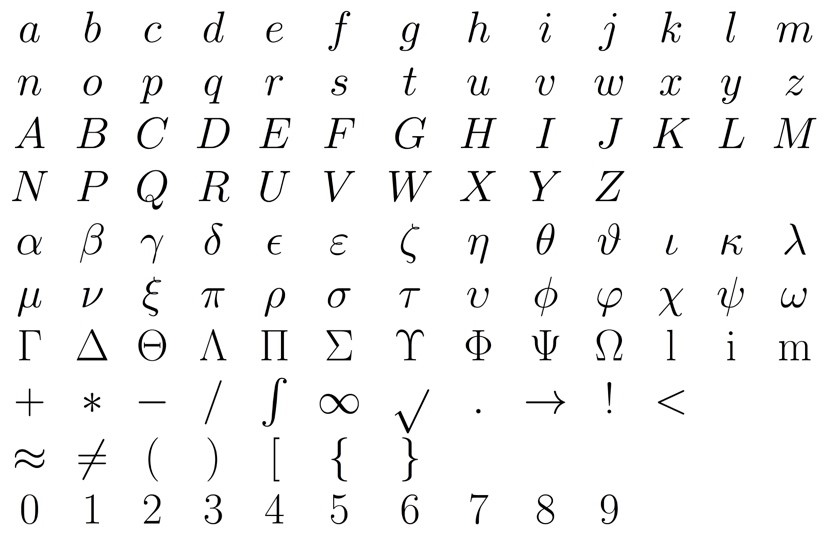
\includegraphics[width=\columnwidth]{palette}
    \caption{Character Palette}
    \label{fig:palette}
\end{figure}

Then, we classify each character found by the segmentation algorithm through a nearest neighbor classifier using “cityblock” distance, which produced the best results compared to other types of distances, and we output the best match as the detected character. This along with the centroid and bounding box with respect to the original equation are passed to the equation assembly function.

\subsection{Equation Assembly}
We assemble each equation sequentially from left to right using each recognized character’s bounding box. Notably, as we process each character, we keep track of a “previous” centroid to detect the presence of superscripts and subscripts. This is not just the centroid of the previous matched character in the case of a fraction, where the "previous" centroid is really the centroid of the fraction bar. The basic flow of the algorithm is as follows:

If the current character’s bounding box does not overlap with any subsequent bounding boxes, we add the character to the equation directly using the following rules:
\begin{enumerate}
    \item If the lower-left corner of the bounding box is above the height of the “previous” centroid, either a superscript or the end of a subscript has occurred. We keep track of a subscript flag to differentiate the two.
    \item If the upper-left corner of the bounding box is below the height of the “previous” centroid, we carry out the opposite operation from above.
    \item Otherwise, if the character is a \LaTeX control sequence, $\backslash$ is pre-appended to the character and a space is post-appended. Then the aggregate is added to the equation.
    \item Otherwise, the character is added directly with no modifications.
    
\end{enumerate}

If the current character overlaps with subsequent bounding boxes, we check for specific cases:
\begin{enumerate}    
    \item If the character is '-' and only overlaps with another '-', we append a ‘=’ to the equation and skip the overlapping '-'.
    \item If the character is a square-root, we grab all of the subsequent overlapping characters and recursively assemble a sub-equation. Then, we append the appropriate \LaTeX command to the total equation.
    \item If the character is '-' and does not only overlap with another '-':
    \subitem If the width of the ‘-‘ is a large portion of the width of the union of the overlapping bounding boxes, we recognize the overlapping region as a fraction. We divide the characters into  denominator and numerator sets and then recursively assemble these two sets into sub-equations. Finally the fraction is assembled into the proper \LaTeX format and appended to the total equation.
    \subitem Otherwise, it is a negative sign, and we continue to the next cases.
    \item We look for a limit-enabled control sequence (summation, integration, and product), and then recursively assemble the equations of the upper and bottom limits as appropriate.
\end{enumerate}

This logic is limited in the number of \LaTeX constructions supported. For example, we do not support all of the numerous \LaTeX control sequences. Also, variable modifiers such as the dot or bar notation will not be correctly assembled.

\section{Results}
The binarization method yielded no problems on our test cases. Compared to performing Otsu’s method Adaptive Thresholding, using our heuristic implementation runs in about half the time. The results are shown in Table \ref{tab:deskew_results}.


\begin{minipage}{\columnwidth}
    \captionof{table}{Time for Deskewing on Demo\_equation.jpg} \label{tab:deskew_results} 
    \begin{tabularx}{\columnwidth}{|X|X|X|}
        \hline
        & 10 Runs &	20 Runs \\
        \hline
        Otsu’s Method &	5.743720 seconds &	11.529060 seconds\\
        \hline
        Mean Threshold	& 11.232951 seconds &23.221652 seconds\\
        \hline
    \end{tabularx}    
\end{minipage}

\begin{figure}[!t]
    \centering
    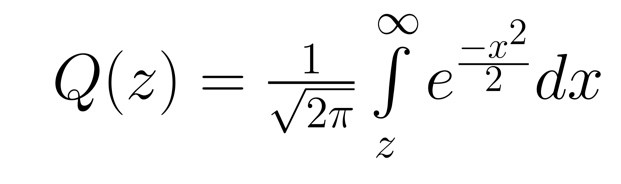
\includegraphics[width=\columnwidth]{clean}
    \caption{Sample "Clean" Equation}
    \label{fig:clean}
\end{figure}

We also performed derotation tests on our fifteen "clean" equations. This "clean" set was obtained by taking screenshots of direct \LaTeX compilations. See Figure \ref{fig:clean} for an example. We manually rotated each "clean" equation by an angle and ran the derotation algorithm on the resulting image. We then defined the error to be the absolute value of the difference between the detected angle and the rotated angle. The results are graphed in Figure \ref{fig:deskew_graph}. Our algorithm resulted in errors below 2 degrees in magnitude for most of our test equations. Equation 3 is the outlier. This equation was shown above in Figure \ref{fig:1}. Despite the guards described in the Derotation section, our algorithm still registers the diagonal division bar as the dominant orientation for most rotation angles.




\begin{figure}[!t]
    \centering
    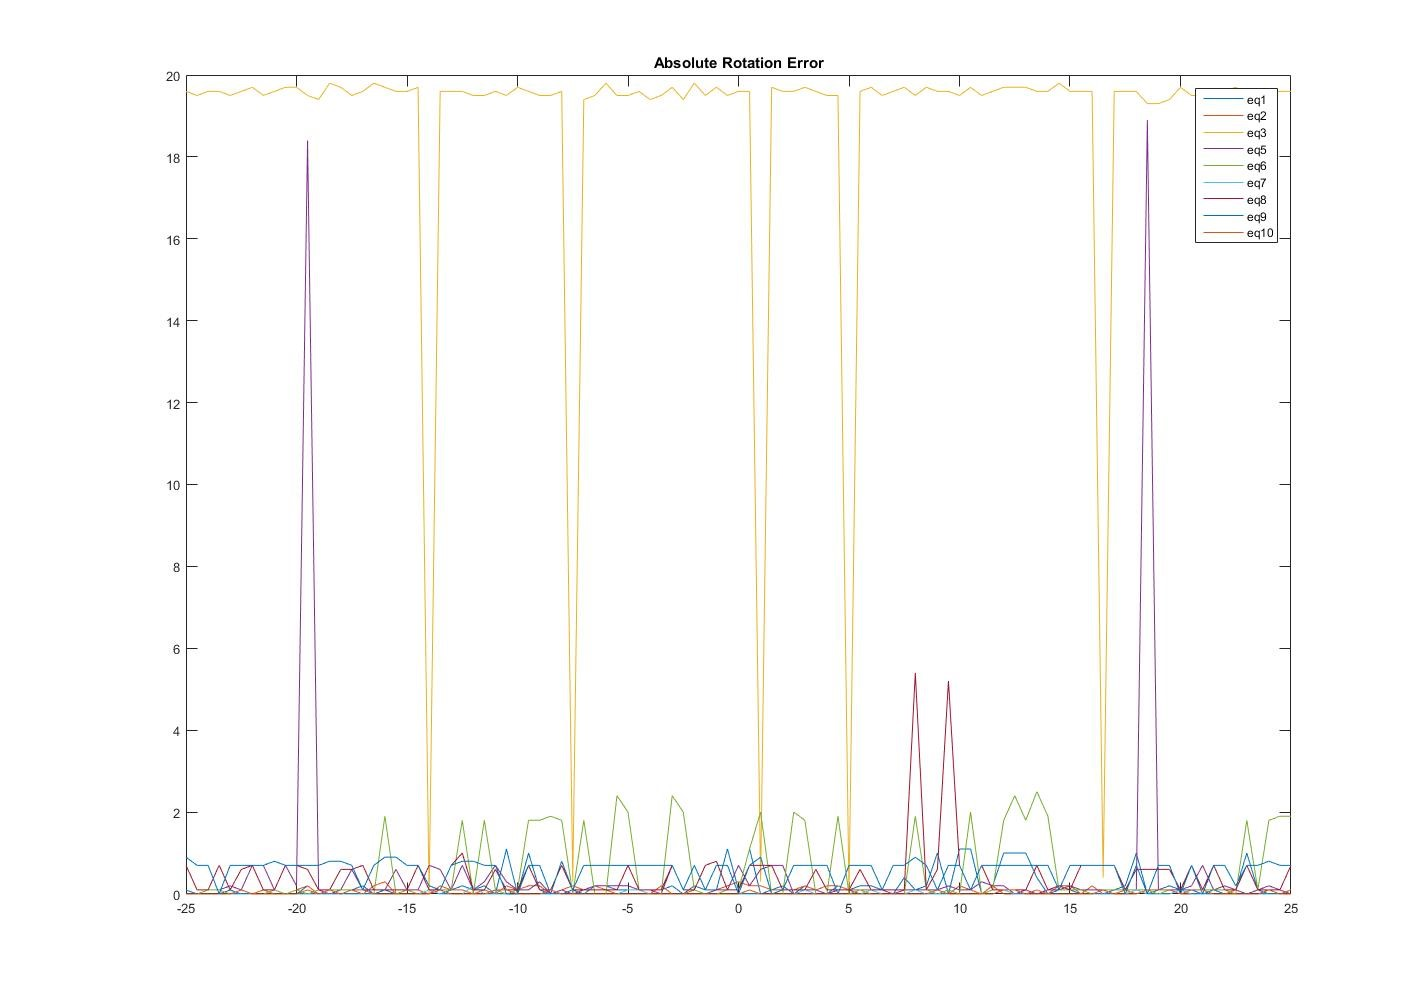
\includegraphics[width=\columnwidth]{deskew_results_graph}
    \caption{Derotation Error}
    \label{fig:deskew_graph}
\end{figure}

We also tested the matching algorithm in several ways. First, the database characters were rescaled before performing character matching. Over a scale range of $0.5$ to $1.25$ the overall correct percentage was $95.3\%$ as shown in Table \ref{tab:scaling_results}.

\begin{minipage}{\columnwidth}
    \captionof{table}{Robustness to Scaling} \label{tab:scaling_results} 
    \begin{tabularx}{\columnwidth}{|X|X|X|}
        \hline
        \textbf{Scale} & \textbf{\# Correct} & \textbf{\% Correct}\\
        \hline
        \hline
        \textbf{0.5} &	103/116 &	88.8\%\\
        \hline
        \textbf{0.75} &	111/116 &	95.7\%\\
        \hline
        \textbf{1.0}	 & 116/116 &	100.0\%\\
        \hline
        \textbf{1.25} &	112/116 &	96.6\%\\
        \hline
    \end{tabularx}    
\end{minipage}

Next, we ran the full pipeline on the fifteen equations in the “clean” set. We observed a matching performance of 147/157 characters for a rate of 93.6\%. The missed characters are partly from false positives and partly from an equation that was incorrectly derotated due to the presence of a $\Lambda$ which acted like the division bar in the test equation in Figure \ref{fig:1}.
We also tested the overall system for robustness to rotation. The fifteen clean equations above were rotated from $-25^\circ$ degrees to $+15^\circ$ in increments of $5^\circ$, and the entire process was run on each rotated equation.

\begin{figure}[!t]
    \centering
    \includegraphics[width=\columnwidth]{rotation_robust}
    \caption{Robustness to Rotation}
    \label{fig:rotation_robust}
\end{figure}

Figure \ref{fig:rotation_robust} shows the detection percentage throughout the rotation test. The overall matching percentage is not significantly affected, except at $10^\circ$ where the deskewing algorithm again was confused by a specific image.

Finally, the algorithm was tested on ten photographs of equations under uneven lighting with a skew, such as in Figure \ref{fig:test_img}. Again, the deskewing method would sometimes be confused by odd characters or by the "$\backslash$" division symbol and "=". We investigated a modification to our deskewing algorithm in which we kept only the dominant Hough peak rather than considering the top four peaks. This modification actually handled the "$\backslash$" worse but handled the odd characters better. The modified and final algorithm produced recognition rates of 98/123 for 79.7\% 91/123 for 74\%, respectively. Combining the best equation results from these two methods gave a combined result of 86.2\% correctly matched characters.

\begin{figure}[!t]
    \centering
    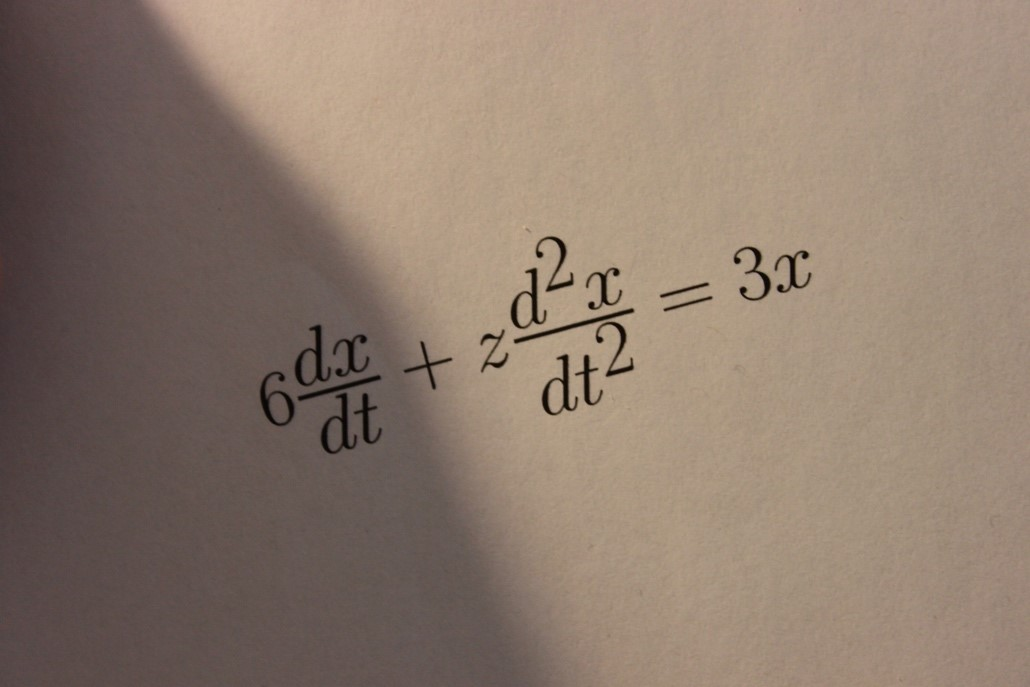
\includegraphics[width=\columnwidth]{test_img}
    \caption{Sample Test Image}
    \label{fig:test_img}
\end{figure}

\section{Limitations}
The deskewing algorithm presented the most limitations. Most of these limitations manifested only in short equations where diagonal lines in characters were dominant enough to outweigh the horizontal lines in the Hough space. However, in practice, this could be overcome by underlining each equation by hand. In fact, this would be a very reasonable augmentation for extending this project to handwritten equations.  

Also, our current character palette for character matching is limited due to the huge variety of \LaTeX characters available. Our process is modular enough that adding additional characters would be simple; we would just add the character to the palette with the appropriate label and the algorithm would proceed as usual. However, we would need to perform additional validations to ensure that no aliasing effects would be introduced. In the same vein, our equation assembly algorithm is limited to recognizing certain patterns. However, in this case, additional \LaTeX equation patterns should be easy to implement.
However, one major limitation of the assembler is fractional exponents. As seen in Figure \ref{fig:clean}, the fraction in exponent is very large. Our current algorithm correctly detects the exponent, and even the nested exponent, but it fails to detect that the following “dx” is outside of the exponent. Therefore, we have imposed the constraint that all fractions within exponents must occur at the end of the exponent, and the algorithm will automatically end any exponent after a fraction is appended. Further work must be done to remove this limitation.

\section{Further Work}
Relevant future additions to our algorithm include the ability to detect and extract an equation from a page with background text and clutter. The current algorithm only supports equations with completely empty backgrounds.

This program has also been architected to be readily extended to recognize handwritten equations. We chose the features for character matching to be invariant to scale and rotation to support the huge variances in handwriting. Possible next steps towards supporting handwritten equations include machine learning to train a linear predictor. This would require the gathering of a training data set rather than a single character palette, but we could use our same feature vector.

Further work can also be done to increase the reliability of the current matching algorithm. The matching algorithm exhibits susceptibility to binarized and smoothed characters that were not “perfect” as pdf images. This could be improved by reducing distortion from the binarization algorithm and adding “non-perfect” characters to the template database. 

The robustness could also be improved by implementing a heuristic based error correction algorithm for the matching system. We could experimentally determine characters that tended to produce consistent false positives and take appropriate compensation actions for these characters. For example, we have noticed that the "$z$"  is often misclassified as an uppercase "$Z$". Knowing this, we could add an additional check when detecting the uppercase "$Z$"  before final classification. For example, we could check whether the top is straight or curved.

Finally our algorithm is rather slow. We made some attempts to decrease our algorithms runtime such as implementing the heuristic based adaptive thresholding and investigating frequency based deskewing algorithms\cite{Kaur:article_typical}. However, speed was not an objective in our original project formulation. As the project matures, though, algorithm optimization will become a central goal for practicality. Future tasks related to this include migrating to a compiled language such as C++ and rigorous algorithm analysis.

Finally our algorithm is rather slow. We made some attempts to decrease our algorithms runtime such as implementing the heuristic based adaptive thresholding and investigating frequency based deskewing algorithms (Kaur, Mandip, and Simpel Jindal). However, speed was not an objective in our original project formulation. As the project matures, though, algorithm optimization will become a central goal for practicality. Future tasks related to this include migrating to a compiled language such as C++ and rigorous algorithm analysis.




% use section* for acknowledgment
\section*{Acknowledgment}


The authors would like to thank Professor Gordon Wetzstein for making this project possible and Kushagr Gupta for consulting.



% trigger a \newpage just before the given reference
% number - used to balance the columns on the last page
% adjust value as needed - may need to be readjusted if
% the document is modified later
%\IEEEtriggeratref{8}
% The "triggered" command can be changed if desired:
%\IEEEtriggercmd{\enlargethispage{-5in}}

% references section

% can use a bibliography generated by BibTeX as a .bbl file
% BibTeX documentation can be easily obtained at:
% http://mirror.ctan.org/biblio/bibtex/contrib/doc/
% The IEEEtran BibTeX style support page is at:
% http://www.michaelshell.org/tex/ieeetran/bibtex/
%\bibliographystyle{IEEEtran}
% argument is your BibTeX string definitions and bibliography database(s)
%\bibliography{IEEEabrv,../bib/paper}
%
% <OR> manually copy in the resultant .bbl file
% set second argument of \begin to the number of references
% (used to reserve space for the reference number labels box)
\bibliographystyle{IEEEtran}
\bibliography{Brewer_Sun}


% that's all folks
\end{document}


